\documentclass[a4paper,11pt]{article}

% ---------- Packages ----------
\usepackage[margin=2.5cm]{geometry}
\usepackage{amsmath, amssymb, amsthm, mathtools}
\usepackage{algorithm}
\usepackage{algpseudocode}
\usepackage{enumitem}
\usepackage{graphicx}
\usepackage{booktabs}
\usepackage{hyperref}
\usepackage{xcolor}

\usepackage{tikz}
\usetikzlibrary{automata,positioning,arrows.meta}

% ---------- Theorem Environments ----------
\newtheorem{theorem}{Theorem}
\newtheorem{lemma}{Lemma}
\newtheorem{definition}{Definition}
\newtheorem{proposition}{Proposition}
\newtheorem{corollary}{Corollary}

% ---------- Custom Commands ----------
\newcommand{\R}{\mathbb{R}}
\newcommand{\N}{\mathbb{N}}
\newcommand{\Z}{\mathbb{Z}}
\newcommand{\Alphabet}{\Sigma}
\newcommand{\eps}{\varepsilon}
\newcommand{\set}[1]{\left\{ #1 \right\}}
\newcommand{\abs}[1]{\left| #1 \right|}
\newcommand{\ceil}[1]{\left\lceil #1 \right\rceil}
\newcommand{\floor}[1]{\left\lfloor #1 \right\rfloor}

% ---------- Section Style ----------
\renewcommand{\thesubsection}{(\alph{subsection})}
\renewcommand{\thesection}{}\renewcommand{\thesubsection}{(\alph{subsection})}

% ---------- Algorithm Style ----------
\algrenewcommand\algorithmicrequire{\textbf{Input:}}
\algrenewcommand\algorithmicensure{\textbf{Output:}}

% ---------- Title Info ----------
\title{\textbf{CSE2315 — Assignment 2}}
\author{Vlad Paun \\ 6152937}
\date{\today}

% ---------- Document ----------
\begin{document}

	\maketitle
	%\thispagestyle{empty}
	%\newpage

	\section{Exercise 1}
	Suppose we have the following language $L$ over the alphabet $\Alphabet=\set{a,0,1}$:
	\[
	L = \set{ua^kv | u,v\in \set{0,1}^* \text{ and }c_0(u) + c_1(v) > k}
	\]
	Where $c_x(w)$ is defined as the number of occurrences of $x$ in $w$. Use the pumping lemma to show that $L$ is not regular.

	\begin{proof}By contradiction.\\
		Assume to the contrary that $L$ is regular. Let $p$ be the pumping length given by the pumping lemma. Choose $s$ to be the string $a^p1^p1$. Because $s$ is a member of $L$ and $s$ has length more than $p$, the pumping lemma guarantees that $s$ can be split into three pieces, $s = xyz$, where for any $i \ge 0$ the string $xy^iz$ is in $L$. We show this outcome is impossible.\\
		Condition 3 of the pumping lemma says that $|xy| \le p$. Thus, in the case of our word, y must consist of only $a$s. Let $k_{xyz}$ and $k_{kyyz}$ represent the number of $a$s in $xyz$ and $xyyz$ respectively. $k_{xyz} = p$ and $k_{xyyz} > k_{xyz} = p$, but the number of $1$s in $xyyz$ is still $p+1$. Thus in $xyyz$ we have $c_0(u) + c_1(v) \le k_{xyyz}$, so $xyyz$ cannot be in $L$. Therefore, $s$ cannot be pumped and we have reached our desired contradiction.
	\end{proof}

	\section{Exercise 2}
	Suppose we have the context free grammar $G=(\set{S,T,V},\set{a,b,c},R,S)$, with R containing the following rules:
	\begin{align*}
		S &\to Tc\mid cV\\
		T &\to aTb\mid bTa\mid \eps\\
		V &\to a\mid b
	\end{align*}

	\subsection{Describe the set $L(G)$ in your own words.}
	\subsection{Construct a PDA $M$ such that $L(M)=L(G)$. Use no more than 8 states.}
	\subsection{Explain how your PDA works.}

	\section{Exercise 3}
	Consider the following rules $R$ of a CFG $G = (\set{S,A,B},\set{a,b},R,S)$:
	\begin{align*}
		S &\to bB\mid abB\\
		A &\to bA\mid AA\\
		B &\to AS\mid SA\mid \eps \\
	\end{align*}
	Convert G into Chomsky normal form.\\
	First, we add a new start variable.
	\begin{align*}
		S_0 &\to S\\
		S &\to bB\mid abB\\
		A &\to bA\mid AA\\
		B &\to AS\mid SA\mid \eps \\
	\end{align*}
	Then, we remove the $\eps$-rules.
	\begin{align*}
		S_0 &\to S\\
		S &\to bB\mid abB \mid \textbf{ b $\mid$ ab} \\
		A &\to bA\mid AA\\
		B &\to AS\mid SA\mid \textcolor{gray}{\eps}\\
	\end{align*}
	Third, we remove all unit rules.
	\begin{align*}
		S_0 &\to \textcolor{gray}{S} \mid \textbf{bB $\mid$ abB $\mid$ b $\mid$ ab}\\
		S &\to bB\mid abB \mid b \mid ab \\
		A &\to bA\mid AA\\
		B &\to AS\mid SA\\
	\end{align*}
	Convert the remaining rules into proper form.
	\begin{align*}
		S_0 &\to VB \mid TB \mid b \mid UV\\
		S &\to VB\mid TB \mid b \mid UV \\
		A &\to VA\mid AA\\
		B &\to AS\mid SA\\
		T &\to UV\\
		U &\to a\\
		V &\to b\\
	\end{align*}
	\section{Exercise 4}
	Let $L$ be the set of all TUDON words.
	\subsection{Give a CFG $G$ such that $L(G) = L$, using no more than 6 variables and 9 + 26 rules.}
	Let $G = (\set{S,T,U,V,X},\set{<,>,:,;,a,b,\dots,z},R,S)$, with $R$ containing the following rules:
	\begin{align*}
		S &\to <T>\\
		T &\to U:VX\\
		X &\to ;T \mid \eps\\
		U &\to \Alphabet U \mid \eps\\
		V &\to S \mid U
	\end{align*}
	Where $\Alphabet$ refers to any character $a,b,\dots,z$
	\subsection{Explain why your grammar generates $L$}
	So basically the start variable makes one of those dictionaries, and then defers to a new variable for the contents of the dict. Then that variable T makes a key value pair, appended with an X. Then the X can be nothing, or a semicolon and then another T. And then the actual key is any number of alphabet characters, and the value is also any number of alphabet characters or another dictionary.
	\subsection{Is your grammar ambiguous? Give an example or an argument why not.}
	The grammar is not ambiguous, the only part where it could be ambiguous, is when creating the key-value pairs in the dictionary, you could substitute them and creating them in different orders, but I take care of that by appending them one by one do what is already there. This way, there is no ambiguous word.
	\section{Exercise 5}
	Let the operator $@$ be defined as $A@=\set{a^{|w|}\mid w\in A}$. Prove that regularity is closed under $@$.
	\begin{proof}
		Let $A$ be a regular language. We will prove that $A@$ is also regular.\\
		Since $A$ is regular, there is a DFA $M=(Q,\Alphabet,\delta,q_0,F)$ such that $L(M) = A$. Now we will build the NFA $M'=(Q,\set{a},\Delta,q_0,F)$, where $\Delta(q,a) = \set{\delta(q,x)\mid x\in\Alphabet}$. In other words, take $M$ and replace every symbol on transition arrows with $a$.\\
		Next, we must show that the set of words reachable in $M'$ by reading $n$ $a$s from the input is equivalent (meaning the same lengths of words) to the set of words reachable in $M$ by reading any $n$ characters from an input word. This can be shown using induction. It is left as an exercise to the reader.
	\end{proof}
	\section{Exercise 6}
	\subsection{Let $N$ be an arbitrary NFA with $k$ states. Explain why if $L(N) \neq \emptyset$, then there is a word of length $\le k$ in $L(N)$.}
	If $L(N)\neq \emptyset$, then $N$ must recognize some word. This means that there must be a path from the starting state to some accepting state given by a set of transitions. More formally, take any $w\in L(N)$,where $w = w_1w_2\dots w_m$. There must be a sequence of states $r_0,r_1,\dots,r_m$, such that $r_0$ is the starting state, $r_m$ is an accepting state, and for all $0 \leq i < m$, $r_{i+1}\in\delta(r_i,w_{i+1})$. Now, if $m \leq k$, we are done. However, if $m > k$, then by the pigeonhole principle some state must be repeated. So, in the sequence $r_0,\dots r_x,\dots,r_x,\dots,r_m$,we can remove everything between the $r_x$s, including one of the $r_x$s themselves, and we can keep doing this procedure until the length of the sequence becomes $\leq k$. Now, this sequence exactly describes an input word of length $\leq k$ that is in $L(N)$.
	\subsection{Led $D$ be an arbitrary DFA with $k > 1$ states. Give a counterexample to the claim that there is a DFA $D'$ with $k-1$ states, such that $L(D') = L(D)$.}
	Let D be the DFA described by the following state diagram (assume the alphabet is $\set{a,b}$):\\
	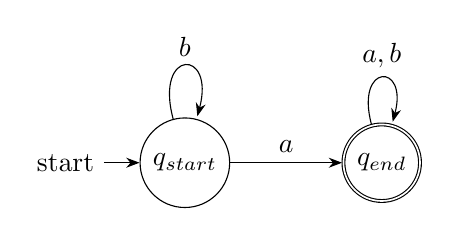
\begin{tikzpicture}[->, >=Stealth, auto, node distance=2.5cm]
		\node[initial,state] (qstart) {$q_{start}$};
		%\node[state] (q2) [right of=qstart] {$q_2$};
		\node[state, accepting] (qend) [right of=qstart] {$q_{end}$};

		\path (qstart) edge node {$a$} (qend);
		\path (qstart) edge [loop above] node{$b$} (qstart);
		\path (qend) edge [loop above] node {$a,b$} (qend);

		%\path (qstart) edge node {$a \cup b \cup abb$} (q2);
		%\path (q2) edge node [below]{$\varepsilon\cup b$} (qend);
		%\path (q2) edge [loop below] node {$a\cup b \cup bbb$} (q2);
	\end{tikzpicture}\\
	This DFA only recognizes words that contain at least one $a$ inside. If we were to construct a DFA with $k-1$ states, it would have to have 1 state. This state could either be accepting, or not. Which means $D'$ would either accept every word, or no words. Neither of which are equivalent to $D$.
	\section{Bonus Exercise}

\end{document}